\documentclass[noindent]{ctexart}
\usepackage{graphicx}
\usepackage{caption}
\usepackage{subcaption}
\usepackage{geometry}
\geometry{left=1.5cm,right=2.5cm,top=2.5cm,bottom=2.5cm}
\CTEXsetup[format+={\flushleft}]{section}

\begin{document}
\section*{ECEI分类结果说明}
\subsection*{分段平均处理}
利用物理系那边提供的读取序列的脚本,得到的序列长度为$9900000$,如图\ref{fig:subfig:original}。
\begin{figure}[h]
    \centering
    \begin{subfigure}[b]{0.45\textwidth}
        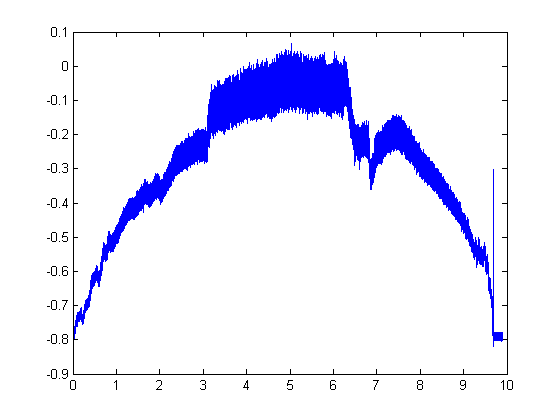
\includegraphics[width=\textwidth]{495.PNG}
        \caption{原始序列}
        \label{fig:subfig:original}
    \end{subfigure}
    ~ %add desired spacing between images, e. g. ~, \quad, \qquad, \hfill etc.
      %(or a blank line to force the subfigure onto a new line)
    \begin{subfigure}[b]{0.45\textwidth}
        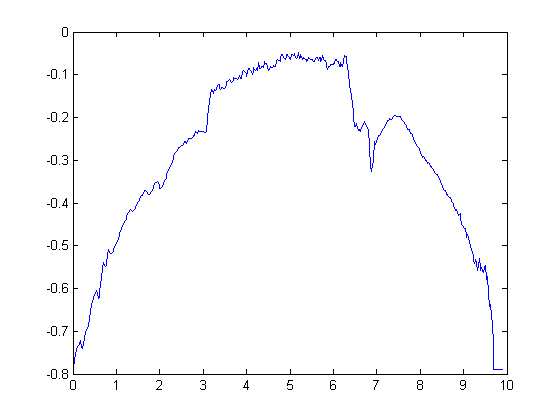
\includegraphics[width=\textwidth]{20000.PNG}
        \caption{分段平均处理后的新序列}
        \label{fig:subfig:new}
    \end{subfigure}
    \caption{序列分段平均处理能提取序列的信息}\label{fig:add}
\end{figure}

可以看出,序列的波动很大,经过每$10000$取平均的分段平均处理后,得到序列长度为$990$,如图\ref{fig:subfig:new}。

分段平均处理能够去除序列的扰动的影响,得到的新的序列能够概括原始序列的关键信息,而且重要的是,分段平均处理能够极大降低计算量。

\subsection*{DTW分类}
分类利用warp window大小为5\%的DTW方法,首先选择SHOT$49024$为测试集,其他已标记好的SHOT为训练集,用$1$NN分类,因为计算量很大,只得到了SHOT$49024$的部分分类结果,未得到的结果均以$NaN$表示。比较分类结果和SHOT$49024$的标记,可以看出:
\begin{itemize}
 \item 大部分情况下,能够正确对label为$1$(good)的序列分类,也就是说能够分开good和bad两种类型的序列。
 \item 对于三种bad类型的序列,label为$2$(saturate)的序列一般都会被正确分类。label为$-1$(weak (bad)	
)的序列总是被错分成$0$(no signal (bad)),这点需要进一步克服。
\end{itemize}

然后再对无标签的SHOT$57241$分类,得到的一小部分分类结果见附录。

\end{document} 